\documentclass[man]{apa2}
\usepackage{pslatex}
\usepackage{amssymb}
\usepackage{graphicx}
\usepackage{color}
\usepackage{covington}
\usepackage[usenames,dvipsnames]{xcolor}
\usepackage{booktabs}
\usepackage{setspace}


\title{Understanding the effect of social context on learning: \\ A replication of Xu and Tenenbaum (2007b)}

\twoauthors{Molly L. Lewis}{Michael C. Frank}
\twoaffiliations{Department of Psychology, Stanford University}{Department of Psychology, Stanford University}


\abstract{Does the source of a piece of data influence the inferences drawn from that data? Xu and Tenenbaum (2007b) find that it does: When a category exemplar is presented from a knowledgable teacher, learners generalize more narrowly than when it is presented from an unknowledgable source.  In five experiments---four online and one in-person---we attempt to replicate this result. We replicate the original result but find an effect size much smaller in magnitude than the original. 

~\\

Keywords: word learning, induction, Bayesian inference}

\shorttitle{Replication of Xu and Tenenbaum 2007b}
\rightheader{Replication of Xu and Tenenbaum 2007b}

\acknowledgements{ 

~\\

\noindent Address all correspondence to Molly L. Lewis, Stanford University, Department of Psychology, Jordan Hall, 450 Serra Mall (Bldg. 420), Stanford, CA, 94305. Phone: 650-721-9270. E-mail: \texttt{mll@stanford.edu}}

\begin{document}

\maketitle       

\section{Introduction}
Imagine you were on a hike and saw a rock positioned oddly at an ambiguous intersection of trails. If you thought you were on a trail which no one had traveled in years, you probably wouldn't think much of that rock. But, if you knew your campmate had traveled that same trail earlier that day, you might interpret the rock differently: You might interpret the rock as a sign intended to point you to the correct path. This intuition---that the source of a piece of information influences the strength of the inference to be drawn---suggests that social information may have a privileged role in human learning.

\citeA{xu2007} examine this phenomenon in the context of a particularly difficult inductive problem: Concept generalization in word learning. Faced with a novel word and its referent, children must decide between an infinite number of hypotheses about the concept extension of that word. For example, consider a child who hears the word ``banana'' in the context of a single banana on a table. While the referent of that object is clear in the moment of language use (i.e., the particular banana on the table), the broader concept is highly ambiguous: ``banana'' could refer to the category of bananas, the category of fruit, that particular species of banana (e.g., plantains), yellow things, or any number of other ad-hoc categories. 

\citeA{xu2007} ask whether children make use of the information source of a new word to guide their inferences about how to generalize its meaning. In particular, they test a prediction that falls out of their word learning model. In their model, learners observe data as word-object pairs and make inferences about the concept associated with that word from a hypothesis space of all possible meanings. Critically, the model predicts that an ideal learner should generalize more broadly when the exemplar is sampled from the full hypothesis space of meanings ({\it weak sampling}), and should generalize more narrowly when the exemplar is sampled from only the true concept of the word within the full hypothesis space ({\it strong sampling}). 

In their experiment, \citeA{xu2007} manipulate sampling ``strength'' through the presentation source of the data. The learner is either presented with three exemplars of the target word from a knowledgeable teacher or the learner makes (correct) guesses about the referent of the word. Importantly, in both conditions, the data that the participants observes is the same: three exemplars from the same subordinate category. What differs is the strength of the sampling. Since the teacher knows the true concept, the data are sampled strongly from the true concept. But, in the learner-generated condition, the learner is naive about the true underlying concept and thus the data are sampled weakly from the full hypothesis space. The key prediction is that, given a hypothesis space with hierarchical concepts (basic, subordinate, superordinate; i.e., banana, plantain, fruit), participants in the teacher condition should be more likely to generalize broadly to the basic level, while participants in the learner condition should generalize conservatively to only the subordinate condition. Their data support  this prediction in both adults ($d = 1.49\ [0.01,\ 2.97]$) and children ($d = 1.21\ [.19,\ 2.23]$).

There are a number of reasons to conduct a replication of this study. First, attempted replications for other predictions of this model have challenged this framework. In a different paper, \citeA{xu2007word} use the same model to make predictions about the effects of another factor in the learning context: the number of observed exemplars. Thier model predicts that a learner should generalize more narrowly when given three observations of a subordinate category, compared to just one (the ``suspicious coincidence effect''). Across three experiments, they find both adults and children behave consistent with this prediction. A number of follow-up experiments have challenged this result, however \cite{jenkins2015non,spencer2011}. Second, recent work has revealed large individual variability across participants in the strength of their sampling assumptions \cite{navarro2012sampling}, making the strength and consistency of the original finding somewhat surprising. Third, this study relies on a social manipulation that is grounded in the interaction between experimenter and participant; such social manipulations tend to have a lower reproducibility rate \cite{reproProj2015}, perhaps due to difficulties in consistently creating the same context and interaction.

% Consider the radically different meaning of observing flowers growing in a meadow versus flowers received from your partner on Valentine's Day. 
Finally, this study is important to replicate because the broad theoretical question---how the source of information influences learning---has far-reaching implications for our understanding of human learning. Every datum is observed in some context, and social aspects of that context can radically change the interpretation of that datum. \citeA{bonawitz2011double} provide a powerful demonstration of this effect. They find that children interpret evidence about the functionality of a toy differently, depending on whether it was taught by a knowledge or unknowledgable teacher. In their experiments, children explore additional  functions of a toy less when a function was demonstrated by a knowledgable teacher, compared to unknowledgable teacher. This suggests that children in the knowledgable teacher condition assumed that there were no additional functions associated with the toy, and thus generalized more narrowly than those in the unknowledgable teacher condition. More generally, evidence such as this suggests that the source of an observation is likely an important factor in learning, and this may be an important factor in the question of how learners make inferences about the world, more generally.

Thus, given the challenges to the \citeA{xu2007a} result, as well as its theoretical significance, we sought to replicate it. We conducted five replications of \citeA{xu2007}, four online (Exp. 1, 2,  4 and 5) and one in-person (Exp. 3). Our data replicate the original effect, but suggest an effect much smaller in magnitude than the original report. In the General Discussion, we suggest a number of factors that may influence the magnitude of this effect that should be explored in future work.
 
\section{Experiment 1} 
In Experiment 1, we attempted to replicate the original design in an online paradigm. 

\subsection{Methods}
\subsubsection{Participants} 
The original sample with adults included 14 participants. We recruited 294 adult participants online through Amazon Mechanical Turk. Participants were paid US \$0.25. 
\subsubsection{Stimuli}
We created four sets of objects similar to the original stimuli (Figure \ref{fig:stims}, left).\footnote{All stimuli, experiments, raw data and analysis code can be found at \url{https://github.com/mllewis/xtSamp}. The analyses can be viewed directly here: \url{http://rpubs.com/mll/xtSamp}.} There were four basic level categories that included 15 unique objects each. Within each basic level category, there were three subordinate categories, with 5 unique objects each. The same novel words were used as the original experiment: ``wug,'' ``tupa,'' ``blicket,'' and ``fep.''
\begin{figure}[t]
 \begin{center} 
 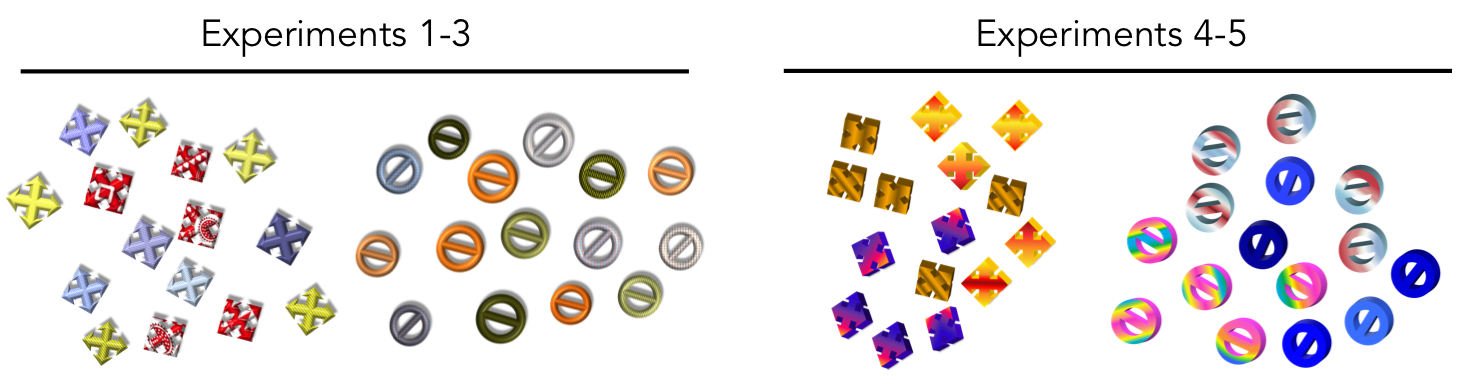
\includegraphics[width=5in]{figures/stims.png} 
 \caption{ \label{fig:stims} Sample stimuli used in Experiments 1-3 (left) and Experiment 4 and 5 (right). The Experiment 4 and 5 stimuli are intended to be maximally similar to the original Xu and Tenenbaum (2007b) stimuli, with lower subordinate-level variability than the stimuli used in Experiments 1-3. All stimuli can be accessed here: \url{https://github.com/mllewis/xtSamp/tree/master/experimentMaterials/stimuli}. } 
 \end{center} 
\end{figure}	
 
\subsubsection{Procedure}
 \begin{figure} [t]
 \begin{center} 
 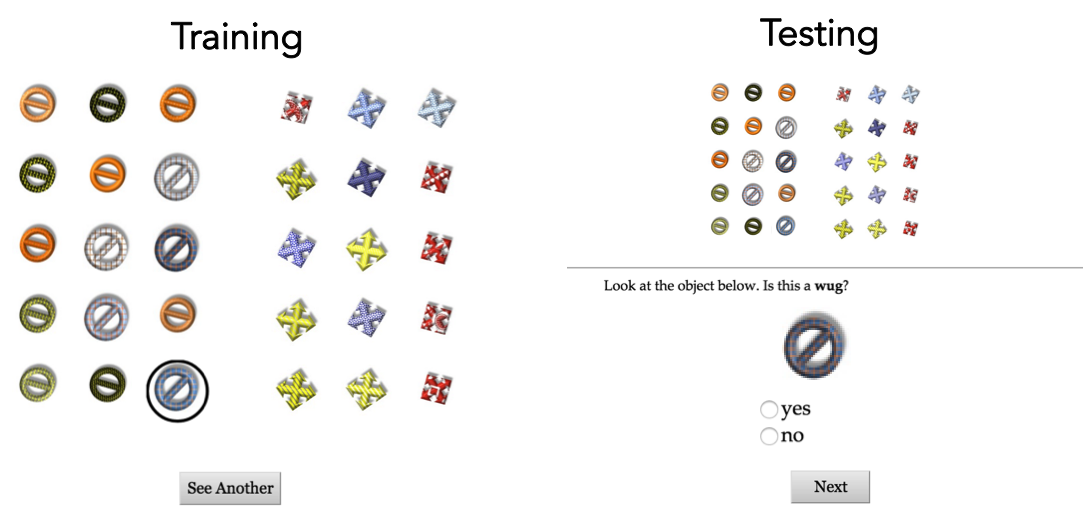
\includegraphics[width=5.5in]{figures/screen.png} 
 \caption{\label{fig:screen} Screen shots of the training (left) and testing (right) phases in Experiment 1. } 
 \end{center} 
\end{figure}


Participants first viewed an instruction page that described the task. In the teacher condition, the instructions read: 
\begin{quote}
In the first part of the experiment, you will see pictures of objects. Some of the objects are called \textit{wugs}. In order for you to learn which objects are \textit{wugs}, I will circle three of them for you. After you learn about the \textit{wugs}, you will be asked questions about them.
\end{quote}
In the learner condition, the instructions were identical except the second sentence above was replaced with: ``In order for you to learn which objects are \textit{wugs} you will try to find two of them. I will tell you whether you are right or wrong.''

Participants then viewed a screen showing all the objects from two basic level categories. Within each basic-level category, the shapes were arranged in a 5 x 3 grid, and the two categories were spatially separated (Figure \ref{fig:screen}). One of the objects in the category on the left was circled. In the teacher condition, the instructions read: ``Find the object that is circled below. That object is a \textit{wug}. When you click on the `See Another' button, I will show you another \textit{wug}.'' The participant was then asked to press a button which caused a circle to appear around one of the exemplars from the same subordinate category as the initially circled object. The participant clicked the button twice in total. 

In the learner condition, the instructions were identical, except the last sentence was replaced with: ``The object circled below is a \textit{wug}. Click on two more \textit{wugs}.'' Participants were then asked to click on two more objects. After each click, a pop-up window appeared with the text ``You're correct! That's a wug.'' This text appeared regardless of the object the participant clicked on. The display then showed the object with a circle around it to indicate that it had been selected. Critically, in both the teacher and the learner conditions, the final display was identical: Thirty objects from two basic level categories, with three circled exemplars.

Participants then advanced to the test phase. On the test screen, the objects from the training phase were shown at the top of the page in an identical format to the training phase, but without the exemplars circled. Below these objects was a horizontal line, and a generalization question (Figure \ref{fig:screen}). There were five generalization questions presented sequentially in the same order as in the original report (subordinate match, basic non-match, basic match, subordinate match, basic match). In each test question, one of the exemplars was shown with the following text above: ``Look at the object below. Is this a wug?'' Participants responded by marking ``yes'' or ``no'' using radio buttons.\footnote{After these questions, we asked several additional questions related to an additional manipulation irrelevant to the current work.} Finally, we asked an attention check question where participants had to selects the label they previously learned from four alternatives.

Objects categories and word items were randomized across participants. The order of presentation of the individual objects on the screen was also randomized, as was the placement of the first circle. Sampling condition was manipulated between-participants. This and all subsequent online paradigms can be viewed directly here: \url{https://mllewis.github.io/projects/xtSamp/xtSampindex.html}.

\subsection{Results and Discussion}

 \begin{figure} [t]
 \begin{center} 
 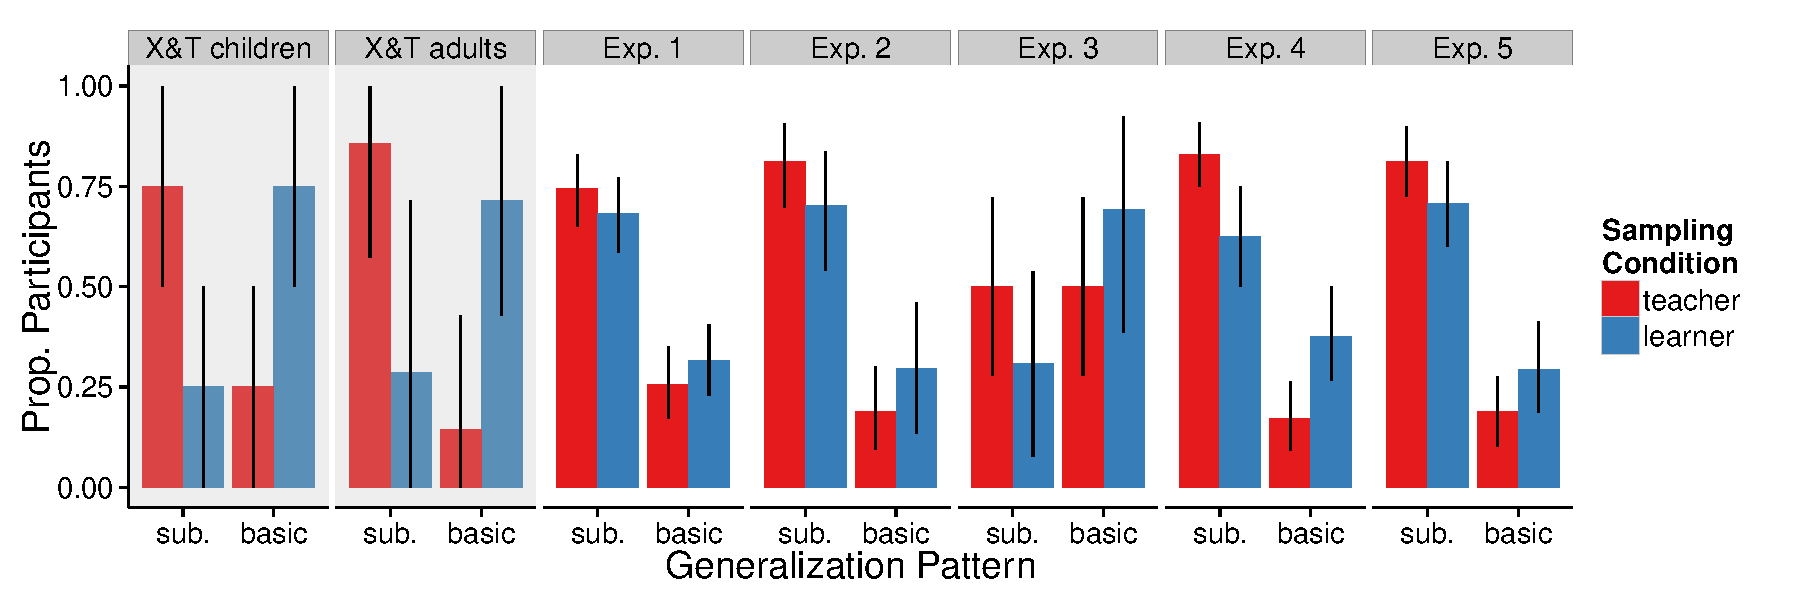
\includegraphics[width=6.2in]{figures/FIG_2.pdf} 
 \caption{\label{fig:bar_plots} Proportion participants generalizing to the subordinate (sub.) or basic level category in the original child ($N = 24$) and adult experiment ($N = 14$), and in our five replication attempts ($N_{1} = 294$; $N_{2} = 150$; $N_{3} = 41$; $N_{4} = 200$, $N_{5} = 500$). Experiments 1, 2, 4 and 5 were conducted online, and Experiment 3 was conducted in-person. Error bars reflect 95\% confidence intervals, calculated via non-parametric bootstrapping. Note that we report the Xu and Tenenbaum data by aggregating across participants, rather than trials (the method in the original report).} 
 \end{center} 
\end{figure}

We excluded participants from our analysis who responded ``yes'' to the basic non-match question ($N=8$) or who did not select subordinate matches in the learning condition ($N = 21$), because this pattern of response indicated a misunderstanding of the task. No participant missed the attention check question. Our final sample included 274 participants ($N_{learner} = 128$; $N_{teacher} = 146$).

In all four experiments, we adopt two different criteria for categorizing participants' response pattern. Unlike in the original report, we found that not all participants responded consistently across questions of the same type within a trial (for example, a participant might respond ``yes'' to one subordinate match and ``no'' to another). Thus, we adopted a liberal criterion which categorized a participant as a basic-level generalizer if they responded ``yes'' to both the subordinate matches and {\it at least one} basic-level match. We also analyzed our data using a strict criterion, where a participant was categorized as a basic-level generalizer if they responded ``yes'' to both the subordinate matches and {\it both} basic-level matches. Under both criteria, a participant was categorized as a subordinate-level generalizer if they responded ``yes'' to only the subordinate level matches. We excluded participants from our analysis who could not be categorized under either criterion. We report the results using the liberal criterion in the Main Text and describe the results using the strict criterion in Appendix A. In no case does the statistical significance of the results depend on the criterion we used. 

Under the liberal criterion, 79 participants could not be categorized as either basic or subordinate-level generalizers, and thus were excluded. While the remaining responses followed the same qualitative pattern as the original, the difference between sampling conditions was not reliable ($\chi^2(1) = 0.63$, $p = .32$; Figure \ref{fig:bar_plots}). The effect size was also much smaller than the original finding ($d = 0.17\ [-0.17,\ 0.51]$; Figure \ref{fig:effect_sizes}).

\begin{figure} [t]
  \centering
  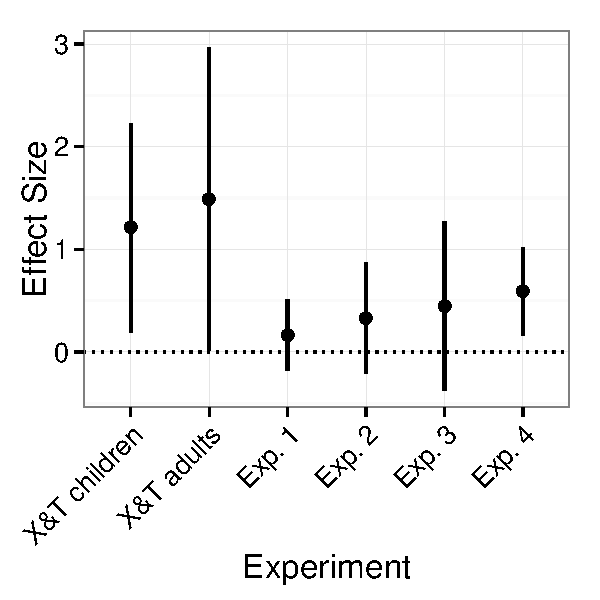
\includegraphics[width=6in]{figures/FIG_3.pdf} 
  \caption{\label{fig:effect_sizes} Effect sizes for the original experiment with children and adults, and our five replication attempts. Effect size estimates are calculated  by transforiming the log odds ratio into Cohen's $d$ (S\'{a}nchez-Meca, Mar\'{i}n-Mart\'{i}nez, \& Chac\'{o}n-Moscoso, 2003; Del Re, 2013). The red diamond indicates the estimate based on a random effect model of all seven studies. Error bars are 95\% confidence intervals.} 
\end{figure}


\section{Experiment 2}

Given that we did not replicate the original effect, we sought to alter our paradigm in Experiment 2 to more closely reflect the original in-person experiments. One critical difference between the in-person and online paradigm is the salience of the experimenter: In the in-person version, the teacher was an actual person interacting with the participant, while in Experiment 1, the reality of the teacher had to be inferred based only on first person text (``I will show you...''). Thus, one reason we might have observed a smaller effect in Experiment 1 is that participants might not have assumed strong sampling in the teacher condition. In Experiment 2, we tried to strengthen this manipulation by introducing the teacher with a picture.

We made also made several other changes to our design. Because many participants in Experiment 1 did not generalize at all (answered ``no'' to all generalization questions), we added questions that queried the original three exemplars that participants learned about. These ``proper name'' trials allowed us to more directly understand these participants' generalization strategy. We also reduced memory demands between the training and testing phases by circling the training exemplars in the testing phase, allowing participants to reflect back on their training data during test.

\subsection{Methods}

\subsubsection{Participants} In Experiment 2, we recruited 150 participants from Amazon Mechanical Turk. Participants were paid US \$0.25 for their participation.

\subsubsection{Stimuli}
The object and word stimuli were identical to Experiment 1.

\subsubsection{Procedure}
The procedure was identical to Experiment 1, with the exception of several key changes described below.

First, we increased the saliency of the experimenter by adding a clipart image of a woman. In the initial instructions, we introduced her by saying, ``Hi, my name is Natalie.'' The image of the teacher was also present in the training and testing phases. These changes were made in both the teacher and learner conditions.

Second, we slightly altered the language of the experimenter to sound more natural. In the learner condition, the instructions in the training phase read: ``Click on two more objects that you think might also be called wugs.'' We also changed the feedback in the training phase to be, ``Yeah, that's a wug.'' In the testing phase, we added the following text above the training items: ``You identified the objects below as wugs'' (the training exemplars were circled, see below). In the teacher condition, the instructions in the training phase read: ``Find the object that is circled below. That object could be called a wug. When you click on the ``See Another'' button, I will show you another wug.'' In the testing phase, we added ``I showed you these objects were wugs'' above the training items. We also changed the critical question to be ``Could this be called a wug?,'' instead of ``Is this a wug?'' in both conditions. This was done to increase the number of basic-level interpretations of the generalization question. 

Third, we added more generalization questions and randomized their order. Each participant was queried about 10 objects in total: The three training exemplars, two objects from the same subordinate level category as the training exemplars, three basic matches, and two basic non-matches. 

Fourth, we reduced memory demands between the training and testing phases by showing the full set of training items during testing (as in Experiment 1) but leaving the selected exemplars circled. This change ensured that participants remembered which objects had been identified as examples of the target category. 

Finally, we added three additional check questions. We showed participants an object from the target category, as well as two objects from never-seen categories. For each of these objects, we asked ``Did you learn about this kind of object?.'' Participants responded by indicating ``yes'' or ``no'' on a radio button.

\subsection{Results and Discussion}
As in Experiment 1, we excluded participants who responded ``yes'' to the basic non-match question ($N=15$) or who did not select subordinate matches in the learner condition ($N = 22$). We also excluded participants who missed any of the attention check questions ($N = 9$). Our final sample included 118 participants ($N_{learner} = 43$; $N_{teacher} = 75$).

The criteria for categorizing a participant's generalization strategy were identical to Experiment 1, except for the inclusion of the additional questions. To be categorized as either a subordinate or basic-level generalizer, a participant had to respond ``yes'' to all training items. To be categorized as a basic-level generalizer, a participant had to respond ``yes'' to one of the three basic-level questions under the liberal criteria, and ``yes'' to all three under the strict criteria. 

An additional twenty-eight participants were excluded because they could not be categorized as a subordinate or basic-level generalizer. For the remaining participants, there was not a reliable effect of sampling on generalization ($\chi^2(1) = 0.89$, $p = .34$; $d = 0.33\ [-0.22,\ 0.88]$). Proportions and effect sizes are shown in Figures \ref{fig:bar_plots} and \ref{fig:effect_sizes}, respectively.

\section{Experiment 3}
Despite increasing the saliency of the teacher, we did not replicate the original effect in Experiment 2. We remained concerned that the teacher was less salient in our version, however, relative to the original. To address this possibility, we next conducted an exact replication of the original study in the laboratory with a real experimenter.

\subsection{Methods}

\subsubsection{Participants} In Experiment 3, we recruited 41 undergraduate participants. Participants received either course credit or payment (US \$5.00) for their participation. 

\subsubsection{Stimuli}
The object and word stimuli were identical to Experiments 1 and 2. 

\subsubsection{Procedure}
The procedure in Experiment 3 closely followed the original. The experimenter presented 15 objects from two basic-level categories on two pieces of paper. On each paper, the objects were spatially unstructured. As in the original, the experimenter asked five generalization questions (see Experiment 1) and each participant completed two trials such that they were trained and tested on two different categories. Participants were incentivized in the training phase with a sticker. The exact script used by the experimenter is in Appendix B. 

\subsection{Results and Discussion}
We excluded one participant who did not select subordinate-level matches in the training phase. We also excluded nine participants because they could not be categorized as a subordinate or basic-level generalizer. Of the remaining 31 participants ($N_{learner} = 13$; $N_{teacher} = 18$), there was not a reliable effect of sampling condition on generalization ($\chi^2(1) = 0.49$, $p = .48$; $d = 0.45\ [-0.38,\ 1.28]$). One notable difference in this experiment, however, was the rate of generalizations to the basic level: In Experiment 3, there were overall more basic level generalizations compared to the online versions. We return to this difference in the General Discussion.

\section{Experiment 4}
Experiment 3 suggests that the decreased effect sizes in the online paradigm were not due the decreased saliency of the experimenter. In the next replication, we explored another possible difference between our experiments and the original: the object stimuli. While similar to the original, our objects had slightly more variability within each subordinate level than the original. This increased variability may have led participants to be less likely to generalize to the basic level. Thus, in Experiment 4, we conducted an online replication using the same procedure as Experiment 2, but with less variable objects at the subordinate-level. 

\subsection{Methods}

\subsubsection{Participants}  We recruited 200 participants from Amazon Mechanical Turk. Participants were paid US \$0.30 for their participation.

\subsubsection{Stimuli}
The objects contained less subordinate-level variability than that used in Experiment 1-3, and were highly similar to the original (Figure \ref{fig:stims}, right).

\subsubsection{Procedure}
The procedure was identical to Experiment 2.

\subsection{Results and Discussion}

As in the previous experiments, we excluded participants who responded ``yes'' to the basic non-match question ($N=17$) or who did not select subordinate matches in the learning condition ($N = 27$). We also excluded participants who missed an attention check question ($N = 10$). Our final sample included 161 participants ($N_{learner} = 69$; $N_{teacher} = 92$).

An additional twenty-one participants were excluded from our analyses because they could not be categorized as a subordinate or basic-level generalizer. Of the remaining sample, there was a reliable effect of sampling on generalization: Participants in the teacher condition were more likely to generalize to the subordinate category, while participants in the learner condition were more likely to generalize to the basic-level ($\chi^2(1) = 6.42$, $p = .01$; $d = 0.59\ [.15,\ 1.03]$). This dataset thus replicates the pattern seen in the original Xu and Tenenbaum (2007b) report, though with a much smaller effect size.

\section{Experiment 5}
In our final experiment, we repeated Experiment 4 with a pre-registered sample size based on the effect size estimated from Experiments 1-4 and the Xu and Tenenbaum adult experiment. 

\subsection{Methods}

\subsubsection{Participants}  To determine the sample size for Experiment 5, we conducted a power analysis based on the effect size estimated from our four replications attempts and the original adult experiment. Based on this  effect size, a sample size of 355 was required  achieve 95\% power on the chi-squared test. Given an approximately 35\% data loss in the previous online experiments, we decided on a sample size of 500 participants. We preregistered our sample size on Open Science Framework (\url{https://osf.io/5xg96/wiki/home/}). As in Experiment 4, participants were recruited on Amazon Mechanical Turk and  paid US \$0.30 for their participation.

\subsubsection{Stimuli}
The stimuli were identical to Experiment 4.

\subsubsection{Procedure}
The procedure was identical to Experiment 4.

\subsection{Results and Discussion}

As in the previous experiments, we excluded participants who responded ``yes'' to the basic non-match question ($N=40$) or who did not select subordinate matches in the learning condition ($N = 63$). We also excluded participants who missed an attention check question ($N = 21$). Our final sample included 408 participants ($N_{learner} = 172$; $N_{teacher} = 236$).

An additional sixty-one participants were excluded from our analyses because they could not be categorized as a subordinate or basic-level generalizer. Of the remaining sample, there was a reliable effect of sampling on generalization: Participants in the teacher condition were more likely to generalize to the subordinate category, while participants in the learner condition were more likely to generalize to the basic-level ($\chi^2(1) = 24.49$, $p <.001$; $d = 0.71\ [.43,\ .99]$).

\section{Meta-analytic Results}
To best estimate the underlying effect size, we used meta-analytic methods to aggregate across estimates from each study. We defined a random effects model  based on the estimates from all seven studies\cite{Viechtbauer2010}. The random effect model treats each effect size estimate as an estimate of an underlying population effect size, and weights it by the precision of the estimate (sample size). 

Across all seven studies, the estimated effect size was .53 ($[.28,\ .78]$; Fig. 4). This estimate was only slightly reduced when the original experiment  with children was excluded  ($d = .50\ [.24,\ .75]$). Thus, while much smaller than the original effect size, we replicate the original effect of sampling on generalization.

\subsection{General Discussion}

Across five replication attempts, we replicate the original result in Experiments 4 and 5. 

LOTS OF MODERATORS
- things that might matter:
* variability visually
* spatial structure
* features of the teacher (reliable?)
- in the learner condition, only in lab shows same pattern as original in sub vs. basic
* cost of getting it wrong (``good enough processing'' - in communication vs. turk) 

% A limitation of this paradigm is that the learner - would be nice to have paradigm where sampling didn't come from learner in learning context (other random way)

The social context of human learning also has practical consequences for the interpretation of data collected in psychological experiments. Experimental data are often consistent with at least two accounts---an account that relies on reasoning about the intention of the experimenter, and an account that relies on context-independent reasoning. Consider two examples. A well-known phenomenon in word learning is that children are biased to select a novel object for a novel word, given the presence of both a familiar and novel object \cite<often referred to as {\it mutual exclusivity} in the literature, >{markman1988}. This pattern is difficult to account for psychologically, however, because there are at least two accounts of this behavior. On the one hand, this result could be due to a context-independent bias to assume that lexicons are structured with one word mapping to one concept, and one concept mapping to one word. Another possibility relies on reasoning about the intentions of the experimenter \cite<Why would the experimenter use a strange word to refer to the familiar object if she meant the familiar one?;>{clark1987principle, clark1988logic}. Both of these accounts make similar predictions, and are therefore difficult to disentangle empirically.

Another example of this interpretative ambiguity is the \citeA{heider1944} study. In this task, participants viewed a short movie showing several geometric shapes moving in a way that appeared to be contingent. Nearly all participants spontaneously interpreted the video as depicting animate beings, rather than as simple shapes moving around. Like in the case of mutual exclusivity, there are at least two ways to interpret this result. One possibility is that participants rely on low level features of the scene to infer animacy (e.g., contingency), but another possibility is that participants infer the intention of the experimenter who created the videos and assume an animate intention. 

These two cases---mutual exclusivity and animacy projection---represent a sample of a pervasive theoretical issue in experimental psychology: Data consistent with both pragmatically rich and context-independent accounts. There is not a simple solution to this empirical challenge because it is impossible to fully eliminate a social context from experimental paradigms. Our best bet, therefore, is to try to understand the influence of the social context on learning, and \citeA{xu2007} represents a insightful attempt to systematically shed light on this practical issue.

\section{Appendix A}

\begin{table}[h]
\centering
\begin{tabular}{rrrrr}
 \hline
 & N excluded & $\chi^2$ & $p$ & $d$ \\ 
 \hline
Exp. 1 & 94 & 0.08 & .78 & $0.09\ [-0.30,\ 0.48]$\\ 
Exp. 2 & 36 & 0.07 & .79 & $0.19\ [-0.46,\ 0.85]$ \\ 
Exp. 3 & 14 & 0.63 & .43 & $0.53\ [-0.35,\ 1.41]$ \\ 
Exp. 4 & 31 & 4.13 & .04 & $0.54\ [0.06,\ 1.02]$\\ 
Exp. 5 & 92 & 17.20 &  .00 & $0.70\ [.36,\ 1.04]$\\ 
 \hline
\end{tabular}
\caption{Results of all five experiments using the strict categorization criteria, described in Experiment 1. ``N excluded'' refers to the number of participants excluded from analyses because they could not be categorized as either basic or subordinate-level generalizers. All $\chi^2$ tests have 1 degree of freedom. }
\label{strictResults}
\end{table}


\section{Appendix B}
Below is the script used by the experimenter in Experiment 3. ``[word]'' denotes a randomly selected novel label. Different labels and objects were used in Trial 1 and Trial 2. 

\vspace{5mm}

{\it Thank you for participating in this study. We're going to play a game that was initially designed for preschoolers, so it may seem a little silly, but just play along. Are you ready to begin?}
\vspace{2.5mm}

\noindent \underline{Training} \\
	Teacher Condition: {\it See this? It's a [word]. See this one? It's a [word]. See this one? It's a [word]. Thank you for paying attention. Would you like to choose a sticker? }
\\
Learner Condition: {\it See this? It's a [word]. Can you point to two other [word]s? If you get both of them right you get a sticker! You're correct! You're correct! Would you like to choose a sticker? }
\vspace{2.5mm}
 
\noindent \underline{Testing} \\
{\it Alright, now I'm going to ask you some questions about [word]s. Are you ready?} \\
$\langle$point to subordinate$\rangle$ {\it Is this a [word]?} \\
$\langle$point to basic non-match $\rangle$ {\it Is this a [word]?} \\
$\langle$point to basic match$\rangle$ {\it Is this a [word]?}\\
$\langle$point to subordinate$\rangle$ {\it Is this a [word]?} \\
$\langle$point to basic match$\rangle$ {\it Is this a [word]?} \\
 
{\it Alright, now I'm going to show you some new shapes. Are you ready?}\\

\vspace{2.5mm}
\noindent $\langle$repeat Training and Testing for Trial 2$\rangle$ \\
\noindent {\it All done! Thank you for participating!}

\nocite{re2013}
\nocite{sanchez2003effect}

\section{Acknowledgments}

We thank Marlene Ade for her help with data collection.


\bibliographystyle{apacite2}
\bibliography{biblibrary}

\newpage
\theappendix 
\end{document}
